\documentclass[a4paper,landscape,12pt]{scrreprt}
\usepackage[left=2cm,right=2cm]{geometry}
\usepackage[utf8]{inputenc}
\usepackage{graphicx}
\usepackage{multicol}
\usepackage{framed}
\usepackage[german]{babel}
\usepackage{supertabular}
\usepackage{fancyhdr}

\newenvironment{Figure}
  {\noindent\minipage{\linewidth}}
  {\endminipage}

\usepackage{tikz}
\usetikzlibrary{automata,positioning}
\usetikzlibrary{arrows}
\usetikzlibrary{trees}
\tikzset{
  treenode/.style = {align=center, inner sep=0pt, text centered,
    },
  arn_n/.style = {treenode, circle, black,  draw=black,
    fill=black, text width=1.5em},% arbre rouge noir, noeud noir
}
\newcommand*\circled[1]{\tikz[baseline=(char.base)]{
            \node[shape=circle,draw,inner sep=1pt] (char) {#1};}}
%opening
\title{Social Network Analysis}
\author{Roland Hediger}
\usepackage{helvet}
\renewcommand{\familydefault}{\sfdefault}
\newcommand{\pic}[2][ ]{
\begin{Figure}
 \includegraphics[width=10cm]{#2}
 \captionof{figure}{#1}
\end{Figure}
}
\newcommand{\dsp}{
\hfill \\
}

\raggedcolumns
\begin{document}
\maketitle

\begin{multicols*}{2}
\tableofcontents
\end{multicols*}
\pagestyle{fancy}
\part{Grundkonzepte}
\begin{multicols*}{2}

\chapter{Grundkonzepte 1} % (fold)
\label{cha:grundkonzepte_1}
\begin{description}
	\item[Was ist ein Knoten?]  \dsp
	\begin{itemize}
		\item Personen
		\item Gruppen
		\item Events
		\item Proteine
	\end{itemize}
	\item[Knotenbezeichnungen] \dsp
	Actor,node,site(Physik, selten gebraucht),vertex.
	\item[Was ist eine Verbindung?] \dsp
	Beziehungen - : \\
	\begin{itemize}
		\item Freundschaft(frei gewählt)
		\item Verwandschaft in einer Organisation (vorgegeben)
	\end{itemize}
	\item[Verbindungbezeichnungen] \dsp
	tie,link,bond,relationship,connection.
\end{description}
\section{Andere Begriffe} % (fold)
\label{sec:andere_begriffe}


\begin{description}
	\item[Edge] Ungerichtete Verbindung (Kante)
	\item[Dyade] Knotenpaaer mit möglicher Verbindung
	\item[Triade] drei Knoten mit möglichen Vebindungen
	\item[Pfad] direkt verbundene Knotenkette
	\item[Geodesic] Kurzeste Pfad
	\item[Clique] Komplett verbundener Subgraph
	\item[Community] Gemeinschaft - keine eindeutige Struktur
	\item[Komponent] allein stehender Teil eines Netzwerks
	\item[Graph] Mathematische Bezeichnung für Netzwerk

\end{description}
% section andere_begriffe (end)
\section{SNA Allgemein} % (fold)
\label{sec:sna_allgemein}

\begin{description}
	\item[Herausforderungen] \dsp
	Begrenzung der Population,Fehlende Datewnpunkte,Rauschen in den Vewrhaltensdaten, Semantik von Verhaltensdaten,Komplexität.
	\item[Analyse Ebenen] \dsp
	\begin{description}
	 	\item[Mikro] Knoten und ihre Umgebung
	 	\item[Meso] Elemente innerhalb eines Netzwerks 
	 	\item[Makro] Gesamte Netzwerk Struktur
	 \end{description}
\item[Metriken] \dsp
\begin{itemize}
 	\item Dichte
 	\item \# bestehende / \# mögliche Verbindungen
 	\item $ \Delta = \frac{\sum_{i,j} x_{ij}}{n(n-1)}$
 	\item Zentralitätsmasse Position v Aktoren
 	\item Graph Korrelation und Regression
 	\item Random und bias nets, QAP EGRM
 	\item Simulationen
 \end{itemize} 
 \item[Hypothesen, Selektion vs Einfluss] \dsp
 Nestzwerkstruktur $\Rightarrow$ Verhalten,Einstellung \\
 Machen mehr freunden glücklicher?
\end{description}
 	
% section sna_allgemein (end)
% chapter grundkonzepte_1 (end)

\chapter{Grundkonzepte 2} % (fold)
\label{cha:grundkonzepte_2}
\section{Eigenschafen von Dyaden} % (fold)
\label{sec:eigenschafen_von_dyaden}
\begin{description}
	\item[Dyadischer Zensus]\dsp
\begin{itemize}
	\item Mutual/ Reciprocal \\
	\begin{framed}
	\begin{tikzpicture}[shorten >=1pt,node distance=1cm,on grid,auto] 
	\node[arn_n] (q_1){}; 
%   \node[state] (q_1) [above right=of q_0] {$q_1$}; 
   \node[arn_n] (q_2) [right=of q_1]{}; 

	\path[<->, thick] 
%    (q_1) edge  node {0} (q_1)
%          edge  node [swap] {1} (q_2)
    (q_1) edge (q_2);
	\end{tikzpicture}
	\end{framed}
	\item Asynchron - eingehend oder ausgehend: 
\begin{framed}
	\begin{tikzpicture}[shorten >=1pt,node distance=1cm,on grid,auto] 
	\node[arn_n] (q_1){}; 
%   \node[state] (q_1) [above right=of q_0] {$q_1$}; 
   \node[arn_n] (q_2) [right=of q_1]{}; 
   \node[arn_n] (q_3) [below=of q_1]{};
   \node [arn_n] (q_4) [right= of q_3]{};
	\path[->, thick] 
    (q_1) edge (q_2);
    \path[<-,thick]
    (q_3) edge (q_4);
   \end{tikzpicture}
   \end{framed}
   \item No tie
   \item Multiplexität - überlappung Freund \& Hilfe
   \begin{framed}
   \begin{tikzpicture}[shorten >=1pt,node distance=1cm,on grid,auto] 
	\node[arn_n] (q_1){}; 
%   \node[state] (q_1) [above right=of q_0] {$q_1$}; 
   \node[arn_n] (q_2) [right=of q_1]{}; 
   \draw[thick,double](q_1)--(q_2);
	\end{tikzpicture}
   \end{framed}
   \item Austausch:
 
   \begin{framed}
        \begin{tikzpicture}[shorten >=1pt,node distance=1cm,on grid,auto] 
	\node[arn_n] (q_1){}; 
%   \node[state] (q_1) [above right=of q_0] {$q_1$}; 
   \node[arn_n] (q_2) [right=of q_1]{}; 
   \path[->,thick] (q_1.140) edge  (q_2.140);
  \path[->,thick] (q_2.200) edge  (q_1.-20);
	\end{tikzpicture}
   \end{framed}
\end{itemize}
\end{description}
% section eigenschafen_von_dyaden (end)
\section{Datenformate} % (fold)
\label{sec:datenformate}
\pic[Datenformate:Linked List]{./img/llist.png}
\pic[Datenformate:Matrix]{./img/matrix.png}
\pic[Matrix Sorting]{./img/matsort.png}
% section datenformate (end)
\section{Datenerhebung} % (fold)
\label{sec:datenerhebung}
\begin{enumerate}
	\item Fragebogen
    \item Beobachtungen
    \item Datenbanken
    \item Verhaltensdaten
\end{enumerate}
\pic[Beispiel Quantatives Mapping]{./img/qmap.png}
% section datenerhebung (end)
\section{Social Media Monitoring} % (fold)
\label{sec:social_media_monitoring}
Continuous analysis of available Social Media Content.
\begin{itemize}
	\item Customebr service issues
	\item Competitor infos
	\item PR Disaster Warning System
	\item Company prepared for social conversations??
\end{itemize}
\begin{description}
	\item[Monitoring Features] 
	\begin{description}
	 	\item[Coverage] types ofd media or geographic markets
	 	\item[Sentiment Analysis] Accuracy at a level varied 59-87\%
	 	\item[Location of conversations] self explanitory.
	 	\item[Volume of Conversations] Conversation count.
	 	\item[Latency] Conversation speed. 
	 \end{description} 
\end{description}
\end{multicols*}
% section social_media_monitoring (end)
\section{Definitions Extra} % (fold)
\label{sec:definitions_extra}
\begin{tabular}{|p{7cm}|p{7cm}|p{7cm}|p{4cm}|}
\hline
\textbf{Term} & \textbf{Definition} & \textbf{Interpretation} & \textbf{Example} \\ \hline
Degree (Most Reachable) & Number of direct relations
to other nodes in the
network. (direction of
connection is ignored) & An actor with high degree
centrality is active and
might have immediate
power / prominence within
a network. & \vspace{0cm}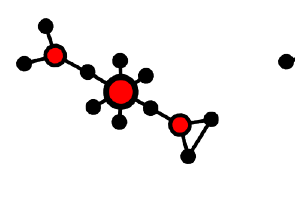
\includegraphics[scale=0.4]{./img/degeg.png}\\ \hline
Closeness(Efficient Reach) & Shortest path distance to
all other actors of the
network (inverse sum).& An actor with high
closeness centrality can
access efficiently all other
nodes in a network.
& \vspace{0cm} 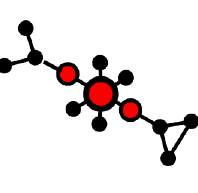
\includegraphics[scale=0.4]{./img/cleg.png} \\ \hline
Betweennness (Control flow) & Number of shortest paths
a node lies between two
other nodes in the
network.& An actor with high
betweenness centrality
can control relations
between others in the form
of preventing or promoting
the flow of information.
&\vspace{0cm} 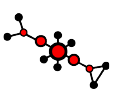
\includegraphics[scale=0.4]{./img/bteg.png} \\ \hline
Eigenvector (Influential Friends) & Importance of a node
based on the connections
of his connections using
the eigenvalue of a node.&
An actor with high
eigenvector centrality
might only have a few
connections but to
strategically important
keyplayers within a
network.& \vspace{0cm} 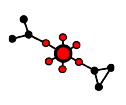
\includegraphics[scale=0.4]{./img/egeg.png}\\ \hline
Clustering(Local Embedded) & Likelihood that two nodes,
which are connected to a
node, are connected
between themselves.An actor with a high
clustering coefficient has
local influence and might
be less susceptive for
outside information.& An actor with a high
clustering coefficient has
local influence and might
be less susceptive for
outside information.
& \vspace{0cm} 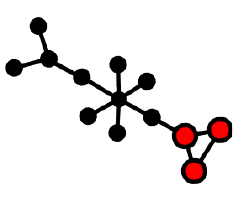
\includegraphics[scale=0.2]{./img/clusteg.png}\\
\hline
\end{tabular}
% section definitions_extra (end)
% chapter grundkonzepte_2 (end)
\begin{multicols*}{2}
\chapter{Grundkonzepte 3} % (fold)
\label{cha:grundkonzepte_3}
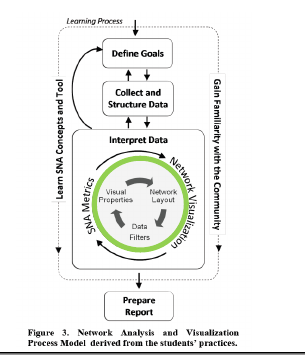
\includegraphics[width=6cm]{./img/mmsna.png}
\section{Arten von Fragestellungen} % (fold)
\label{sec:arten_von_fragestellungen}
\begin{description}
	\item[Knoten Basiert] \dsp
	\begin{itemize}
	 	\item  Sind Mitarbeiter mit mehr Verbindungen erfolgreicher? (Social Capital)
 \item Haben Kunden mit mehr Umsatz auch mehr Kommunikations-Partner?

	 \end{itemize} 
	 \item[Verbindunbgsbasiert] \dsp
	 \begin{itemize}
	 	\item  Führen Freundschafts-Verbindungen zu Business-Verbindungen?
\item  Gibt es einen Zusammenhang zwischen der Migration und dem
\item kommunikations-Volumen zwischen Laendern?
	 \end{itemize}
	 \item[Netzwerkbasiert] \dsp
	 \begin{itemize}
	 	\item Sind Teams mit höherer Kommunikations-Dichte effizienter?
\item Je groesser ein Ego-Netzwerk desto weniger Triaden?
	 \end{itemize}
	 \item[Gemischt] \dsp
	 \begin{itemize}
	 	\item  Beeinflussen sich Freunde gegenseitig in ihrer Meinung zu politischen Themen oder bezüglich Konsumverhalten? (Diffusion, Influence)
 T\item endieren Mitarbeiter dazu bei Personen Hilfe zu suchen, welche
dasselbe Geschlecht haben? (Homophily, Selection)

	 \end{itemize}
\end{description}
% section arten_von_fragestellungen (end)
\section{Zusammenhänge} % (fold)
\label{sec:zusammenh_nge}
\pic{./img/zh1.png}
\pic{./img/zh2.png}
\pic{./img/zh3.png}
% section zusammenh_nge (end)
\section{Kritierien einer guten Visualisierung} % (fold)
\label{sec:kritierien_einer_guten_visualisierung}
\begin{itemize}
	\item Möglichst wenig Überlappungen von Verbindungs-
strukturen (Ausprobieren verschiedener Layoutalgo-
rhythmen und Parameter: Atlas, Fruchterman, etc.)
\item Netzwerk-Komponenten und isolierte Akteure erkennbar.
\item Kategoriale Variablen (z.B. Frau/Mann) werden mit
verschiedenen Farben, Symbolen repräsentiert.
\item Kontinuierliche Variablen (z.B. Anzahl Follower, etc.) sind
mit Grösse, Strichdicke, Farbverläufen dargestellt.
\item Eine Legende der Symbole die Anzahl Knoten und
Verbindungen sind gegebenenfalls ersichtlich.

\end{itemize}
% section kritierien_einer_guten_visualisierung (end)
% chapter grundkonzepte_3 (end)
\end{multicols*}
\part{Mathematischer Hintergrund}
\begin{multicols*}{2}
\chapter{Grundlagen zur Graphen} % (fold)
\label{cha:grundlagen_zur_graphen}
Ein Graph besteht aus Knoten (auch Aktoren oder Nodes genannt) und Kanten (Edges). Im folgenden
kleinen Beispiel-Graphen haben wir die Knoten A bis D. Die Kanten zwischen den Knoten sind hier
ungerichtet was bedeutet, dass die Interaktion in beide Richtungen möglich ist.
Personen C und D zu verschiedenen Teams gehören (z.B Teamleiter sind) und die Person B beide kennt.
In der Sozialen Netzwerkanalyse stellen die Kanten eine direkte oder indirekte Kommunikation /
Verbindung zwischen verschiedenen Aktoren dar. Einer Kante kann dabei verschiedene Bedeutungen
zugetragen werden. Mögliche Bedeutungen:
\begin{itemize}
	\item Informationsaustausch
\item Ressourceaustausch
\item Beeinflussung
\item Mitgliedschafts-Beziehung
\item Verwandschafts-Beziehung
\item Persönliche Beziehung
usw.
\end{itemize}
Oftmals erhalten die Kanten auch ein Gewicht (z.B. Anzahl Benachrichtigungen untereinander). Bei
solchen Graphen wird auch von \textbf{gewichteten Graphen} gesprochen.
Die Netzwerk-Struktur sowie die Eigenschaften von Knoten/Kanten lassen interessante Analysen zu.
Zum einen bietet die Netzwerk-Struktur bereits viel Potenzial um Schlüsselpersonen durch Berechnung
von Zentralitätsmassen zu erkennen. Zum anderen kann das Netzwerk anhand der vorhandenen
Eigenschaften gefiltert werden.


\begin{description}
	\item[Connected Components] \dsp
	\begin{itemize}
	 	\item Menge von Knoten verstanden die über beliebige Pfade miteinander verbunden sind. Ist ein Teilnetzwerk abgeschnitten, bildet es einen zweiten \textbf{Component}
	 	\item Unterschied Strongly Weakly Connected : jeder Node in \textbf{genau einer Component}
	 	\item Strongly Connected : dass ich alle Knoten entlang der Kantenrichtung erreichen. Hier ein Beispiel:\\
	 	 \pic[Connected Components]{img/ccomp.png}
	 	 \item Components im Beispiel: $\{B,C,D,E\},\{A\},\{G,H\},\{F\}$
	 	  \item Bei Weakly Connected Components wird untersucht, welche Knoten einander erreichen, wobei die
Kantenrichtung ignoriert wird und die Kanten einfach als bidirektional angesehen werden. Im
folgenden Beispiel existieren die Weakly Connected Components:
	 	  \pic[Weakly Connected Comonents]{img/wcomp.png}

	 \end{itemize} 
\end{description}
% chapter grundlagen_zur_graphen (end)
\chapter{Interpretation/Metriken} % (fold)
\label{cha:interpretation_metriken}
\begin{description}
	\item[Actor Zentralität] wichtigkeit einzelner Knoten. "Sichtbarkeit des Aktors", Kontrollmöglichkeiten auf den Informationsfluss.
	\item [Degree Centrality] Kanten die von Knoten weg gehen oder zu einem Knoten führen - direkten Verbindungen zum Nachbar. \textbf{Gerichteten Graphen:} InDegree, OutDegree.\\
	\underline{Normalisierung:} Degree Centrality kann als \texttt{Lokales Mass} angesehen werden. Isolierte sicht. Normalisierung berücksichtigt \textbf{Grösse des Netzwerks}\\
	Für die Normalisierung muss der Degree Centrality Wert des Knotens durch die maximal Anzahl
möglichen Verbindungen dividiert werden. Dies sind:\\
Bei ungerichteten Graphen: n-1\\
Bei gerichteten Graphen: 2(n-1)\\
\pic[Degree Centrality]{img/dcen.png}
\pic[Degree Centrality Normalisiert]{img/dcen1.png}\\
\underline{Interpretation:} Degree Wert = Wahrnehmung / Einfluss / Prestige
\item[Closeness Centrality] Nicht lokales Mass. Berechnet für jenen Knoten, wie effizient von einem Knoten aus alle anderen erreichbar sind. \textbf{Berechnung:} \textit{Inversen der kürzesten Distanzen zu allen anderen Knoten werden aufsummiert}. Zeitintensives verfahren:\\
\pic[Closeness Centrality]{img/ccen.png}\\
$C_c(A) = 1 + \frac{1}{2} + \frac{1}{3} + \frac{1}{3} = \frac{13}{6}$\\
Normalisiert : = $\frac{1}{4}*\frac{13}{6}$\\
Für die Normalisierung wird diese Summe dann noch durch die Anzahl Knoten -1 geteilt.
Formel:\\
$C_c(i) = \sum_{j=0}^{N} [d(i,j)]^{-1}$
\item[Betweennness Centrality] Position innerhalb des ganzen Netzwerkes für alle Knoten.\\
\pic[Betweennness Centrality]{img/bcen.png}
\begin{itemize}
	\item Brokerage Position oder Gatekeeper.
	\item Berechnet für jeden Knoten wie stark sich dieser in einer \textit{Brokerage Position} findet
	\item kürzeste Pfad zu allen anderen gesucht. Liegt der Knoten auf viele dieser kürzesten Pfade desto höher Betweennness Centrality.
	\item Algorithmus:
	\begin{enumerate}
		\item Alle Knoten auf BCW\footnote{Betweenness Centrality Wert} 0
		\item Der kürzeste Pfad zum nächsten Knoten geht über den vorherigen. Deshalb wird der BCW dieses Knotens um 1 erhöht - rekursiv weiter
        \pic{img/bcen1.png}
        \pic{img/bcen2.png}
        Vom ersten zum letzten Knoten finden wir einen Spezialfall. Es gibt zwei kürzeste Pfade! In
diesem Fall wird jedem Knoten auf dem Pfad jeweils 1 / \#kürzeste Pfade addiert. In unseremFall würden wir also allen Knoten 0.5 addieren auf beiden Wegen. Die restlichen Schritte werden nach dem gleichen Schema ausgeführt. Weil es sich um ein
bidirektionales Netzwerk handelt muss ein Knotenpaar lediglich einmal berücksichtigt werden.
	\end{enumerate}
	\item Normalisierung:  Gerichtete Graphen: (n-1) * (n-2)\\
 Ungerichtete Graphen: (n-1) * (n-2) / 2
\item Formel: $C_B = \sum_{s \neq v \neq t \in V}\sigma_{st}(V)$
\item Normalisierung Formel: $C_B(v) =\sum_{s \neq v \neq t \in V} \frac{\sigma_{st}(v)}{\sigma_{st}}$
\end{itemize}

\end{description}

\section{Zentralisierung} % (fold)
\label{sec:zentralisierung}
\begin{description}
	\item[Netzwerk Zentralisierung:]  Wie zentral der Aktor ist anhand von Gegebenheiten oder seiner Position innerhalb des Netzwerks.\\
	Eigenschaften : 
	\begin{itemize}
		\item Masse der zentralste Akteur die Zentralität der anderen Akteure überschreitet.
		\item Auf Max Wert bezögen (Netz-abhängig).
		\item Formel: $\frac{\sum^n_{i=1} |C_x(p*)-C_x(p_i)|}{max \sum^{n}_{i=1} 
|C_x(p*)-C_x(p_i)|}$
\item In Worte gefasst bedeutet die Formel: Es wird im Zähler die Differenz zwischen dem höchsten
Zentralitätswert zu allen Aktor-Zentralitätswerte aufsummiert. Der Nenner bekommt den Wert der
maximal möglichen Differenz. So resultiert immer ein Wert zwischen 0 und 1, wobei 0 bedeutet, dass
alle Knoten gleich zentral sind und 1, dass ein Aktor maximale Zentralität besitzt und alle anderen die
tiefste Zentralität. Es besteht also die höchst mögliche Ungleichheit.
	\end{itemize}
	\item[Degree Zentralisierung] Ausgehend von den \textbf{nicht-normalisierten Degree Centrality Werten, berechnet sich in einem ungerichteten Graphen}\\
	\textbf{Formel:} $C_D = \frac{\sum_{i=1}^n |C_D(p*)-CD(p_i)|}{(n-1)(n-2)}$\\
	\textbf{Nicht normalisiert} \\
	\underline{Im fall von einem gerichteten Graph muss der Nenner mit 2 multipliziert werden}
	\item[Betweenness Zentralisierung] \textbf{Geht von bereits normalisierten Aktor zentralitäten aus}\footnote{Alle variablen in diesem Abschnitt mit Strich representieren normalistierte Werten}\\
	\textbf{Formel:} $C_B = \frac{\sum^n_{i=1} |C'_B(p*)-C'B(p_i)|}{n-1}$
	\item[Closeness Centralisierung] \dsp
	\pic{img/nformel.png}
	\textbf{Guter Formel:} $C_c = \frac{\sum_{i=1}^n |C'_c(p*)-C'_c(p_i)|}{\frac{n-2}{2}}$
\end{description}
% section zentralisierung (end)
\section{Metriken} % (fold)
\label{sec:metriken}
\begin{itemize}
	\item Kennzahlen zur komplette Netwerkstruktur
	\item Netwerkvergleich
	\item Schlussfolgerungen ziehen
	\item Kommunikation im Zentrum
	\item Indrekte Kommunikation proportional zum Manipulationsgefahr.
\end{itemize}

\begin{description}
	\item[Graph Density] Wie gut der Graph insgesamt verbunden ist.\\
	Wert zwischen 0 und 1\\
	\textbf{Density für gerichteten Graphen:} $ \frac{|E|}{|V|(|V|-1)}$\\
	\textbf{Density ungerichteten Graphen:} $\frac{2|E|}{|V|(|V|-1)}$\\
	Dichte gibt Auskungt daruber wie schnell sich Informationen in einem Netwerk verbreiten da in einem dichten Netwerk die Kommunikation sehr direkt verläuft und sich somit schnell verbreiten kann. Die dichte nimmt mit der Grösse des Netzwerks ab da der direkte Kontakt zu einer kleineren Menge von leuten gepflegt werden kann, aber nicht zu einer grossen Menge.
	\item[Graph Diameter] "längste kürzeste Pfad" zwischen alle Knotenpaaren in einem Grapgen.\\
	Mehrere Componenets = unendlich \\
	\pic{img/diam.png}\\
	Auskunft über Entfernung der Knoten. Maximale Knoten auf kurzesten Pfad um einen Aktor zu erreichen.
	\item[Cluster Coefficient] \dsp
	\begin{itemize}
		\item Cliquebuildung - 1 ist max Wert - Clique.
		\item Lokalen vs Globalen Cluster Coefficient. Global = Mittelwert von lokalen Werten.
		\item \textbf{Formel:} Quptoienten der Anzahl Kanten zwischen den Nachbarn eines Knoten (\textbf{ungericteten Netwerken mit 2 multipliziert}). und der maximal Anazahl Kanten möglich. \\
		$C_i = \frac{2n}{k_i(k_i-1)}$\\
		\textbf{Globale Clustering:} $C' = \frac{1}{N} \sum^N_i C_i$\\
		\pic{img/ccoef.png}\\
		\begin{itemize}
			\item $C_A = 1$
			\item $C_B = 1/3$
			\item $C_C = 0$
			\item $C_D = 0$
			\item $C_E = 1/3$
			\item $C_F = 0$
			\item $C' = 1/6*5/3 = 5/18$
		\end{itemize}
	\end{itemize}
\end{description}
% section metriken (end)
\section{Communities} % (fold)

\begin{itemize}
	\item Subgraph innerhalb Graphen, stark ziemlich direkt verbunden
	\item Zeigt vertrauensverhältnis
	\item Cliquen haben rendundanten Informations-lieferanten.
	\item Cliquen von innovationen abgekoppelt.
	\item Identifizierung eine Community :
	\subitem Alle kennen einander (Direkte Beziehung)
	\subitem Alle Knoten haben mindestens k Links zu anderem Knoten. (K Core, Gtad der Verbundenheit)
	\subitem Individuellen erreichen einander mit max n Hops (n-Clique).
\end{itemize}

\begin{description}
	\item[KCore] k-Core hat eine weniger einschränkende Bedingung als Clique. Hier muss jeder Knoten mindestens k andere Knoten des Clusters verbunden sein.\\
	\pic{img/kcore.png}
	\pic[3 core Beispiel]{img/3core.png}
	\item[n-cliques] Alle innerhalb einer n-Clique erreichen einander mit maximal n Hops. Eine 1-clique wäre somit eine Clique wie sie vorher dargestellt wurde, wo jeder jeden direkt erreichen kann. Im folgenden Graphen befinden sich drei 1-Cliques, wobei die Knoten B,C und D zu zwei Cliquen gehören:
	\pic{img/nclique.png}
	\pic{img/nclique2.png}
	\begin{itemize}
		\item Durchmesser kann grösser sein als n. Grun ist 2 Cluque.
		\item Knoten von n Clique können z.B nichz mit einander verbunden sein. Roten und Grünen können als 2 Cliques interpretiert werden (rechts).
	\end{itemize}
	\item[p-Cliques]  Bei p-Cliques muss mindestens ein Bruchteil p (Angabe zwischen 0 und 1) aller Kanten eines Knotens zu anderen Knoten führen, welche sich im Cluster befinden. Somit werden viele der oben erwähnten Nachteile beseitigt.
\end{description}

\section{Clustering und Communities} % (fold)
\label{sec:clustering_und_communities}
\begin{description}
	\item[Hierarchical Clustering] Bottom up Clustering verfahren. Jeden Knoten bildet einen eigenen Cluster am Anfang. Zusammenfassung des Graphens Schritt für Schritt. Bei jeder iteration werden die Ähnlichkeiten zwischen allen Clusters untersucht. Stopp bei gewünschten Anzahl Clusters oder alle Knoten befinden sich im selben Cluster.
\end{description}
\underline{Beispiel:}\\
\pic{img/hcb.png}\\
Zu Beginn bildet jeder Knoten seinen eigenen Cluster, es existieren also 8 Clusters. Jetzt werden
diejenigen Knoten zusammengeführt, welche am meisten kommunizieren. Das sind die Knoten A und
B:
\pic{img/hcb1.png}
Nun werden die Knoten D und G zusammengefasst. Da diese nun einen neuen Cluster bilden muss die
Kommunikation zwischen dem neuen Cluster und aussenstehenden Knoten aktualisiert werden. Beide
Knoten kommunizieren mit dem Knoten F. Deshalb muss beim neuen Cluster für die Kommunikation
mit dem Knoten F die Summe zwischen den Knotenpaaren G und F (1) sowie D und F (3) verwendet
werden:
\pic{img/hcb2.png}
\pic{img/hcb3.png}
\pic{img/hcb4.png}
\\
\\
\begin{description}
	\item[Edge Betweennness Clustering]Edge-Betweenness Clustering
Das Edge-Betweenness-Clustering, auch bekannt unter dem Girvan-Neuman Algorithmus, ist ein Top-
Down Clustering Verfahren. Dies bedeutet, dass sich zuerst alle Knoten im selben Cluster befinden und
dann sukzessive aufgeteilt werden.
Wie der Name bereits vermuten lässt wird als Ähnlichkeitsmass der Edge-Betweenness Centrality Wert
berechnet. Die Centrality-Berechnung ist genau dasselbe wie bei der Node Betweenness Centrality,
nur jetzt halt für Kanten. Ein hoher Edge-Betweenness Wert bedeutet, dass es sich um eine Kante
zwischen zwei Knoten-Gruppen handelt. Es gibt wieder mehrere Iterationen, wobei in jeder Iteration
diejenige(n) Kante(n) mit dem höchsten Betweenness-Wert entfernt wird, bis schlussendlich die
gewünschte Anzahl Clusters erreicht worden ist. Dieses Verfahren ist sehr rechenintensiv, da nach
jeder Iteration die Edge-Betweenness Werte neu berechnet werden müssen, der komplette
Algorithmus liegt in $O(n^3)$. Deshalb wird es selten eingesetzt.
Hier ein Beispiel für das Betweenness Clustering. Die Kante(n) mit dem höchsten Betweenness-Wert
sind jeweils rot eingefärbt und werden nacheinander entfernt:
 \pic{img/ebc1.png}
 Nachdem die Kante mit dem höchsten Betweenness-Wert entfernt wurde, werden die Kanten-
Betweenness Werte neu berechnet:
\pic{img/ebc2.png}
\end{description}
% section clustering_und_communities (end)
% section communities (end)
% chapter interpretation_metriken (end)
\chapter{Small World} % (fold)
\label{cha:small_world}
\section{Experimente} % (fold)
\label{sec:experimente}
\begin{description}
	\item[Milgram]Ursprüngliches Paket-Experiment von Milgram
Im Jahre 1967 hat Stanley Milgram folgendes Experiment durchgeführt: 60 Teilnehmer der USA
mussten ein Paket an eine festgelegte Person in Boston, die sozial und geografisch weit von der
Ursprungs-Person entfernt war, ein Paket zusenden. Sie durften es aber nur der Person direkt zustellen
falls Sie diese auch persönlich kennen und mit Vornamen ansprechen. Ansonsten mussten sie es einer
bekannten Person mit gleichem Kriterium weitersenden, bei der die Wahrscheinlichkeit hoch war, dass
sie die Zielperson kennt. Der Weg des Paketes wurde protokolliert. So wurde untersucht, wie viele
Personen zwischen Absender und Empfänger lagen (Anzahl Hops)
Die durchschnittliche Pfadlänge lag bei 5.5. Daraus schliesst sich, dass im Durchschnitt innerhalb der
USA jede Person jede andere über 6 Personen erreichen kann. Es entstand auch der Ausdruck Six
Degrees of Separation Theorie für dieses Phänomen. Dieser Ausdruckt wurde jedoch nie von Milgram
verwendet.
\item[Erdos] Co-Authorship Experiment von Paul Erdős
Ein weiteres Small World Experimente wurde vom Mathematiker Paul Erdős durchgeführt. In einem
Graphen stellt er alle Autoren von Publikationen als Knoten dar. Kanten zwischen zwei Knoten wurden
erzeugt, wenn diese gemeinsam eine Publikation verfasst haben (Co-Autor). Paul Erdős gab sich selbst
die Erdős-Zahl 0. Personen, mit denen er publiziert hatte, erhielten die Zahl 1. Autoren, welche mit Co-
Autoren von Paul Erdős eine Publikation verfasst haben die Zahl 2 usw.
Autoren, welche nicht erreicht werden konnten, erhielten die Zahl „unendlich“. Es zeigte sich, dass die
Zahl entweder unendlich oder sehr klein war. Bei 268‘000 Personen konnte ein endlicher Wert
ermittelt werden, der Durchschnitt bei 4.65 lag. (Erdős hat in sehr vielen Teilen der Mathematik
publiziert).
\item[MSN]Microsoft analysierte 90 Millionen täglich aktive Messenger-Accounts. Jeder Account wurde als Knoten
und die Kommunikation zwischen zwei Personen als Kanten dargestellt. Die Analyse ergab
schlussendlich, dass zwei beliebige Personen durchschnittlich 6.6 Schritte voneinander getrennt
waren. Es gab auch Pfade bis zu einer Länge von 29 Schritten. Damit wurde die Theorie der Small World
anhand eines riesigen, globalen Netzwerks bestätigt, auch wenn die beiden Forscher Eric Horvitz und
Jure Leskovec eher „Seven Degrees of Separation“ als Mass vorschlagen würden. 
\end{description}
\newpage
% section experimente (end)
\section{Eigenschaften} % (fold)
\label{sec:eigenschaften}
\begin{itemize}
	\item  Wenige Hops um Leute zu verbinden
	\item Neigen nahezu Cliquen zu formen
	 \item Hub Nodes (Indegree/Outdegree viel)
	 \item Die Distanz zwischen zwei zufällig gewählten Knoten entspricht etwa dem Logarithmus der Anzahl
Knoten. Duncan Watts and Steven Strogatz haben entdeckt, dass Graphen anhand zwei unabhängigen
Metriken klassifiziert werden können: Clustering Coefficient, Average Shortest Path
\item \textbf{ Um zu erkennen, ob es sich um ein Small-World Graphen handelt} werden die beiden Masse mit einem
Random-Netzwerk mit ungefähr gleicher Degree-Verteilung verglichen. Für ein Small World Netzwerk
sind dann die folgenden beiden Eigenschaften erfüllt:\\
$ L_{SW}  \le L_{RAND}$\\
$CC_{SW} \le CC_{RAND} $
\end{itemize}
% section eigenschaften (end)
% chapter small_world (end)
\end{multicols*}
\end{document}
